\chapter{More on the Linux desktop and Getting started with Moodle}
\newcommand{\moodle}{\textsf{Moodle}}
\newcommand{\Moodle}{\textsf{Moodle}}
\begin{note}
  This is the fifth, two hour, lab.

  There was a feeling that the getting started with Moodle material might be a little light for a 2 hour session, so perhaps put some more Desktop oriented material in here as well.

  Has change of position (?) of this lab made any difference to how we tell students about first tutorial?

  Do we need some breakout boxes in this script?
\end{note}


\section{Getting started with \moodle}
\label{sec:introduction-moodle}

In this lab session you will be introduced to the web application \moodle\ which supports COMP10120. You should also use this lab session to complete the \emph{Individual Learning Profile} questionnaire which is hosted inside \moodle.

\moodle\ is a \emph{Virtual Learning Environment} (VLE) that allows the classroom to extend onto the web. It is not designed to replace face-to-face teaching, but to support it with a range of flexible on-line tools, as well as providing a place to upload resources for course units. Each course unit supported by \moodle\ typically has a single course unit site within the \moodle\ environment.

%Why is Moodle being used for COMP10120
\moodle\ has several features which make it well suited to supporting this course-unit. These include:
\begin{itemize}
\item Providing communication tools for you to easily get in contact with your tutors, other students in your tutor group, and share information with all students on the course unit.

\item Providing a wiki tool which you will use to collaboratively document your project work

\item Providing a structure to help organise activities you should be doing on a week-by-week basis.
\end{itemize}

Now login to \moodle\ by pointing your web browser at: \urlnop{moodle.cs.man.ac.uk}

Your username and password is the same as your University account username and password. Enter these into the login box and select the Login button. If you had problems logging in, check that the caps lock key on your computer keyboard is off and that you use the correct combination of lower case and capital letters in both your username and your password. If you still have problems, speak to a lab demonstrator.

After successfully logging into \moodle\ for the first time, you will be presented with a web form to complete the details of your \moodle\ profile. Add your first and last names; your email address; the city/town where you live (for most people this will be Manchester); and add a short description of yourself. Select the Update profile button to complete your \moodle\ registration. Assuming you have made no errors when completing your \moodle\ profile, the next page to appear will be the \moodle\ home page (see  Figure~\ref{figure:moodle-home})

\begin{figure}
\centerline{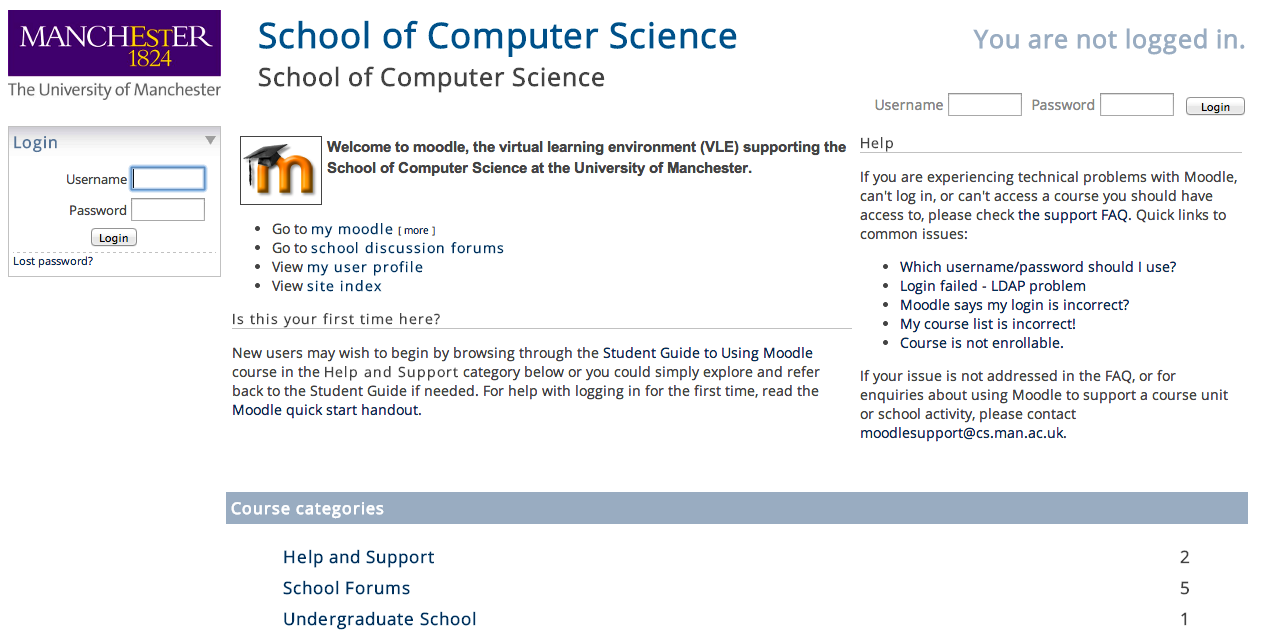
\includegraphics[width=15cm]{images/moodle-home}}
\caption{Moodle Home Page}\label{figure:moodle-home}
\end{figure}

At this stage, you may find it useful to browse though (or at least be aware of) the \emph{Getting started with \Moodle} guide which is deliberately located outside the \moodle\ environment should you run into problems. You can find it at: \urlnop{octette.cs.man.ac.uk/moodleintro} (see Figure~\ref{figure:moodle-start}).

\begin{figure}
\centerline{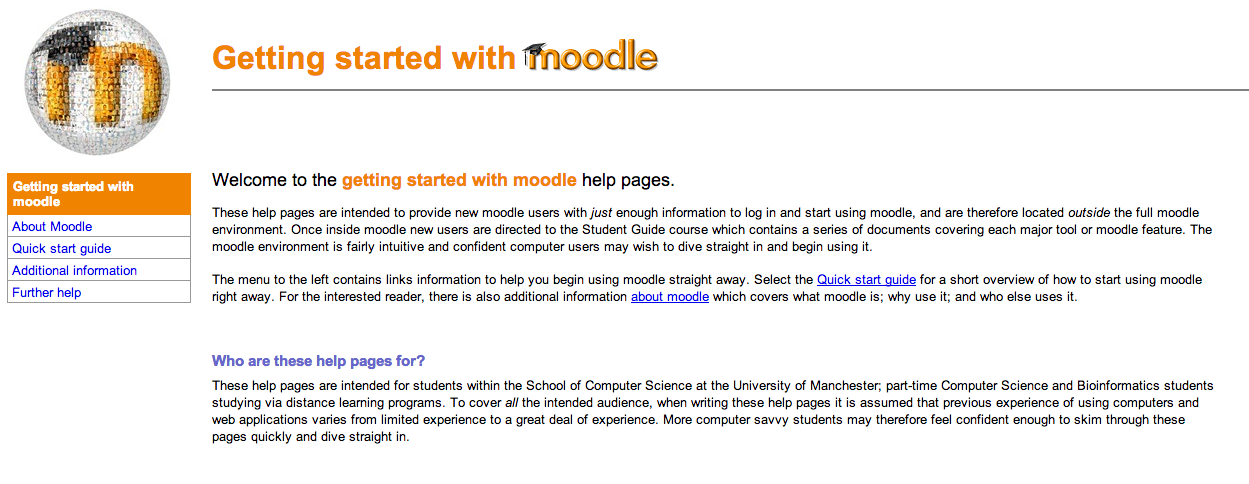
\includegraphics[width=15cm]{images/start-moodle-page}}
\caption{Getting started with Moodle}\label{figure:moodle-start}
\end{figure}



\subsubsection*{Brief overview of the \moodle\ home page}
\label{sec:brief-overv-moodle}


The \moodle\ home page lists several categories in which \moodle\ course unit sites are organised (make sure you scroll down to see them all). \moodle\ course unit sites exist for many, but not all, course units within your degree programme. There are also a number of \moodle\ sites which provide support to staff and students in other ways, such as a general CS help sites and the Staff Student Consultative Committee public site.

You can find links to sites by either locating the link in the appropriate category, for example look in \emph{Undergraduate School/First Year} for COMP10120; or you can enter \emph{COMP10120} into the \emph{Search courses} field at the bottom of the course list and select the course unit title from the search result(s).

Other things to look out for on the front page include the link to your \moodle\ user profile and the link to the \emph{my moodle} feature. We'll come back to these later on...


%Your turn


Make sure you can find the COMP10120 course unit site and are able to access it. To get back to the \emph{\moodle\ home page} you should click on the \moodle\ link in the navigation bar underneath the course unit title at the top of the page. This is always the first element in the link trail. If you navigate further into the course unit site, to return to the \emph{course unit site front page} just click on the COMP10120 link in the navigation bar. This is always the second element in the link trail.

Now locate the course titled \emph{Student Guide to Using Moodle} (in the category \emph{Help and Support}). Have a browse through what help material is provided here. You may wish to revisit this site to learn how to use one of the \moodle\ activities or understand one of \Moodle's features.

\subsection{The COMP10120 course unit site}
\label{sec:comp10120-course-uni}


If you haven't already, navigate to the COMP10120 site and start to look at how the site is structured and what tools have been provided (see Figure~\ref{figure:101-moodle-page}).
Things you should note about the structure of the site:

\begin{figure}
\centerline{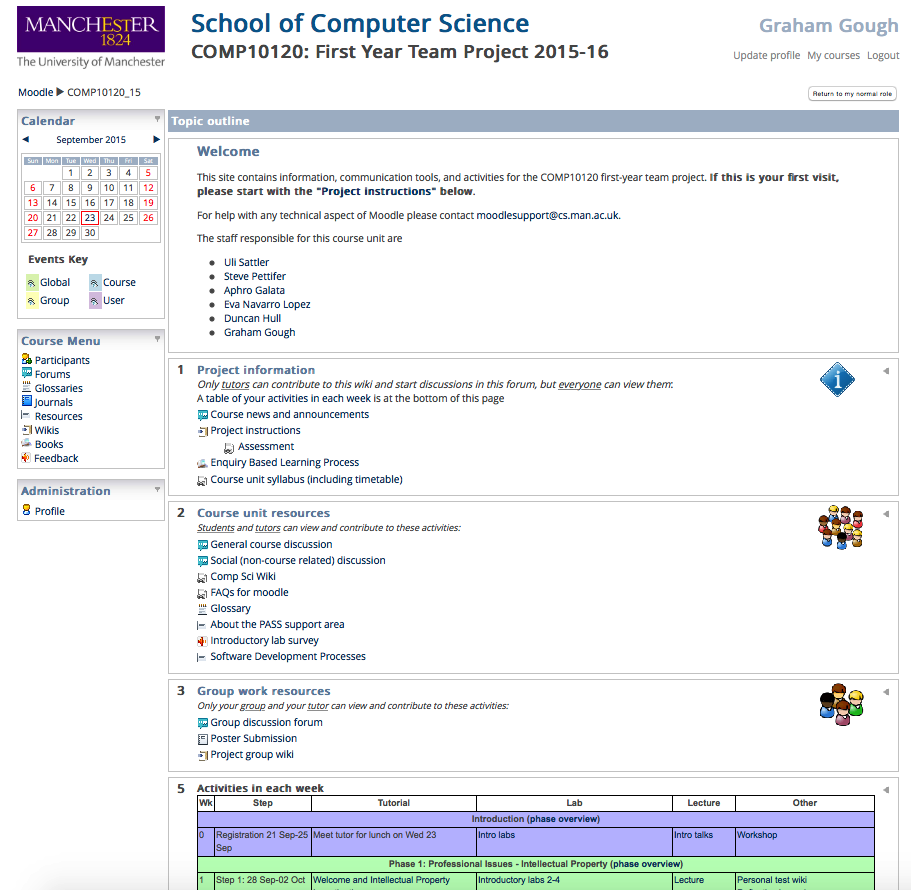
\includegraphics[width=15cm]{images/101-moodle-page}}
\caption{COMP10120 Moodle Home Page}\label{figure:101-moodle-page}
\end{figure}


\begin{itemize}
\item 
All instructions for the course unit are located in the \emph{Project information} area towards the top of the site. Take a look at each of the links in this area. In particular, familiarise yourself with the front page of the \emph{Project instructions} and read at least the \emph{Introduction to the tasks and activities} (and then click through to the \emph{Phases and Tutorials} page to get an idea of the course unit structure).

\item Back on the course unit site, the next section is called \emph{Course unit resources}. If you have a query about the course unit which you think everyone should know the answer to, please use link to the \emph{Question and Answers} site, or browse the existing questions and answers tagged with \emph{comp101-team-project} 

\item The next section is called \emph{Group work resources}. This is your tutor group's area and should be used to communicate with members of your team (by using the forum) and to document your work (in the wiki).

\item Finally, the bottom of the course unit site has a table of all your activities for this course-unit. The different phases are colour-coded to help you spot the one you want. The row for each week contains links to information about what you should be doing in that week and tools/resources applicable to the week. (Don't forget to read the \emph{phase overview} first.)

  The \emph{Other}  column includes resources for your personal use, that you are expected to complete over the course of the year. In particular you should note the \emph{reflective journals} for each week of the first semester. You are expected to reflect on the questions detailed inside the journal each week.
\end{itemize}

% The remaining instructions for this lab session can be found
% directly within \moodle\ itself. Click on \emph{Introduction to \Moodle} % in the \emph{Lab} column for \emph{Step 1} in the green (\emph{Phase 1}  section.

\subsection{Lab deliverables}
\label{sec:lab-deliverables}

\begin{note}
  Do we want a list of deliverables for each lab? Should they be at the start of the script?
\end{note}

By the end of this lab session, ensure you have completed the following tasks.

\begin{itemize}
\item 
Posted a welcoming message to your tutor group (see Using forums below).

\item Create your set of practise wiki pages (see Using wikis below).

\item Completed the Individual Learning Profile questionnaire
\end{itemize}

There are also a number of optional tasks you should aim to complete if you have time during the lab.

\subsection{Using forums}
\label{sec:using-forums}


Most of you will have used discussion forums in some way or another, whether on your favourite social networking site or on some other website. \Moodle's forums aren't too different to any other, however, you should note a few things:

Most forums are configured so that copies of each posting will be emailed to other course unit members. In a group forum, copies are only emailed to other group members; in a course forum copies are emailed to everyone.

In most cases you will have the option to remove your subscription to such emails. Please don't do this, at least not at the moment.

In your user profile you have the option to receive \moodle\ emails as a single daily digest (recommended) rather than as multiple emails each day.

You might not be able to post messages in all forums. Some forums (e.g. course announcement forums) will only allow tutors to start new topics of discussion, but will allow students to reply to those topics once started.

%Your turn
Visit your Group discussion forum on the COMP10120 site and click on \emph{Add a new discussion topic}  to begin a new discussion thread. Write a short forum posting to introduce you to your other group members and your tutor. Let them know where you are from, tell them a little bit about yourself. Warning: the current in-line HTML in \moodle\ can sometimes misbehave, especially if you try to apply lots of formatting. Therefore concentrate on content rather than presentation.

Note that your discussion posting won't be emailed to the other members of your group until about 30 minutes after you submit the posting. This is to allow time for you to edit it in case you spot a mistake.

If you want to find out more about using discussion forums, look through the \emph{How to use the forums}  help book in the \emph{Student Guide to Using \Moodle} course. There is also a help book called \emph{Using \moodle's HTML editor} which you may also find useful.

\subsection{Using wikis}
\label{sec:using-wikis}


So what is a wiki? A \wikipedia{Wiki}{Wiki} is an on-line tool which allows multiple people to collaborate on the authoring of web content. Every edit, deletion and addition to the wiki is stored, providing a complete history of wiki changes. Old versions of pages and be retrieved and compared to new versions of pages. Wikis are typically edited using a simple mark-up syntax where the focus is on content rather than fancy presentation.

You have almost certainly come across wiki authored content before, one of the most famous examples being wikipedia (\urlnop{wikipedia.org}). Wikis are also frequently used by software development teams to document their project. The ability to look back to previous versions of documents and the ability for multiple authors to collaborate on producing the documentation is particularly useful in such environments.

During COMP10120 you are required to document many aspects of your work using a group wiki provided by \Moodle. \Moodle's wiki isn't as powerful as others you may have come across as it is primarily tailored towards teaching, but it does allow you to use \Moodle's standard in-line HTML editor to help you with formatting.

%Your turn
In the bottom \emph{Resources for individual use} section of the COMP10120 site you will find a link to a wiki called \emph{Personal test wiki} which is private for you and you only. It is provided to allow you to practise how to use \moodle\ wiki syntax before you start using your shared group wiki. If you have used a wiki before then you may find \Moodle's wiki syntax is slightly different to that which you are used to.

For this short exercise you will need to read through some of the help documentation hosted inside \moodle. In a new window or tab navigate to \urlnop{moodle.cs.man.ac.uk} again and enter the \emph{ \emph{Welcome to the Student Guide to Using \Moodle} }course in the \moodle\ \emph{Help and Support}  category (you may be asked to 'enrol' on this course, just select 'Yes'). Scroll down to the section about Wikis and select the \emph{How to use the wiki tool} book.

The aim of this short exercise is to create a simple wiki page with two or three wiki links to other pages; incorporate an image; and attach and link to a binary (non-image) file. It is important that you follow this mini-tutorial through to the end as it will ensure you know how to do all the basic tasks needed to help build your own group wiki during the project.

For the purposes of this mini-tutorial you are asked to create a small wiki about yourself.

Start by opening your Personal test wiki. You will be presented with the \moodle\ editor which won't contain any content yet. Enter a title for the page, something like \emph{About Me} will do.

Select the \emph{Save} button. You should now see the first page of your wiki with the content you just added. Now select the \emph{Edit} tab so that you can add more content.

Create a short bullet list containing the items \emph{My hobbies},  \emph{My music}  and \emph{My files}  Save the page again and check the results, then select the Edit tab again. Now turn the three items into wiki links. To do this, just put a single set of square brackets around each of the terms, like this: \emph{[My hobbies]}  \emph{[My music]}  \emph{[My files]}  Save the page again and look at what just happened. If everything worked correctly each term enclosed in square brackets should now look like this: term? (emboldened text followed by a hyperlinked question mark).

Select the question mark symbol on the \emph{My hobbies} term. Note this opens up a new wiki page called \emph{My hobbies} for you to populate with content. Add some text to describe a few things about what you like to do with your time and then select Save.

This is the basic process by which you build up a wiki into a series of linked pages. Note that at the bottom of the page you just created is a list of \emph{Referring links}  This means \emph{a list of pages that link to this one}  Select the link back to the front page.

In the Student Guide to Using \moodle\ course look at the help book on wikis and read the chapter titled \emph{Unique names for pages}  in particular instructions on how to make the link text different from the linked page name. Now go back and change your first wiki page so that the link to the page \emph{My hobbies} contains the link text \emph{My interests} (but still points to My hobbies). Your list should now contain the items \emph{My interests},  \emph{My music}  and \emph{My files} 

Now go back and select the question mark link for the \emph{My music} link and add some content to this page too. You could write about music you love (or music you hate!).

In the last part of this mini-tutorial, you will need to add a small picture to your wiki and a small file. First we need some files to play with. If you have a small picture that you took yourself, great, you own the copyright on it. Create a small text file using any text editor containing any text you like. If you don't have a picture to use and can not source a copyright free image, you will find a link to an example image in the summary text box of the wiki above the first page. There is also a link to a sample text file there too.

In the Student Guide to Using \moodle\ course look at the help book on wikis and read the chapters titled \emph{Attaching binary files} and \emph{Linking to attached files}  From your wiki's front page select the question mark link for the \emph{My files} link to create its page content. Attach your text file to the page from the wiki's Attachments tab as described in the \emph{Attaching binary files} chapter of the help book. Then return to the edit tab and add the following text:

\emph{Wikis allow users to attach files, such as this one here}  

Turn the word \emph{here} into a link to the text file you just uploaded following the instructions in the \emph{Linking to attached files} chapter of the help book.

Carefully read the chapter of the help book titled \emph{Incorporating images}  Now add the following text and add the image you grabbed earlier below the text.

\emph{Wikis also allow users to incorporate images such as this one.} 

Experiment with changing the alignment of the image as described in the help book.

Finally, browse through the remaining documentation in the Wiki help book so that you have an overview of what other information is there and can refer back to it in the future if needed. If you have any questions about how to use the wiki tool, post a message to the General course unit discussion forum.

\subsection{Individual Learning Profile questionnaire}
\label{sec:indiv-learn-prof}

Before the end of the lab session make sure you complete the \emph{Individual Learning Profile questionnaire}. You will find it in the \emph{Resources for your individual use} section at the bottom of the \moodle\ course unit site. This activity is to help you to reflect so that you can understand your own basic skills and abilities required for your academic life. It may also be looked at by your personal tutor so the School can be better placed to address your particular needs during your time in the School of Computer Science. This information will only be visible to you, to your tutor and to the course unit organisers.

\subsubsection*{Writing your journal}
\label{sec:writing-your-journal}


One of the aims of this course unit is to encourage you to develop the habit of thinking about the way you are learning and working, and trying to identify ways in which these could be improved. The process of reflection is key to this, but is not something that comes naturally to many of us. In most week slots of the course unit site you will find an instance of the Journal activity. The summary text of each journal contains prompts to aid your reflection that week. The journal is very simple \moodle\ tool which provides you with an editable text area supported by \moodle\ HTML editor. Selecting the \emph{Start or edit my journal entry} button opens your journal. Any entries you put into your journal will be completely private to you and your personal course unit tutor. A limited number of the course unit organisers have access to all students journals, but will respect your privacy and will not be looking at them.

At some time towards the end of this week, start your journal entry for the current week and post your answers the prompts provided.

\subsection{What else is on \moodle?}
\label{sec:what-else-moodle}


As well as course unit sites for many of your course units, there are also a number of open-access areas within \moodle. Within the \emph{Support Forums} category you will find a number of sites where you can seek help about specific areas within computer science, e.g. the C / C++? Programmer's Forum. The \emph{Student / Staff Groups} category includes a site where you can post up questions or topics of discussion for the Staff Student Consultative Committee. All these open-access courses are indicated by the guest user icon (a small person icon or a side-on face depending on your chosen \moodle\ theme). Have an explore and see what is there. More open-access site are likely to be added over the year.

\subsection*{Playing and personalising}
\label{sec:play-pers}


If you have time left in the lab session, spend some time personalising your \moodle\ account. Things you could do include:

Uploading a small photo or image to represent yourself to your \moodle\ profile.

%Personalising your my \moodle\ area.

Take a closer look at the advanced options in your \moodle\ profile and investigate what they do (read up about this in the \moodle\ help course books first).

Look ahead on the COMP10120 site to get a feel for what you will be doing over the coming year.

\section{And finally . . . Blackboard!}
\label{sec:blackboard}


You won't be using it for this course-unit, but for your other course-units you may be using a different Virtual Learning Environment - \textsf{Blackboard}. The usual way to access \textsf{Blackboard} is via the \emph{My Manchester page}, and then the \emph{'My Blackboard'} tab. There is also a plentiful supply of information about how to use Blackboard available online.

